%% Beispiel-Präsentation mit LaTeX Beamer im KIT-Design
%% entsprechend den Gestaltungsrichtlinien vom 1. August 2020
%%
%% Siehe https://sdqweb.ipd.kit.edu/wiki/Dokumentvorlagen

%% Beispiel-Präsentation
\documentclass{sdqbeamer} 
 
%% Titelbild
\titleimage{banner_2020_kit}

%% Gruppenlogo
\grouplogo{sdq_logo.pdf} 

%% Gruppenname
\groupname{Architecture-driven Requirements Engineering}

% Beginn der Präsentation

\title[Generierung von UML-Diagrammen
aus PCM-Modellen]{Generierung von UML-Diagrammen
aus PCM-Modellen}
\subtitle{Praktikum Werkzeuge für agile Modellierung} 
\author[Voneva]{Sonya Voneva}

\date[21.\,3.\,2022]{21. März 2022}

% Literatur 
 
\usepackage[citestyle=authoryear,bibstyle=numeric,hyperref,backend=biber]{biblatex}
\addbibresource{presentation.bib}
\bibhang1em

\begin{document}

%Titelseite
\KITtitleframe

%Inhaltsverzeichnis
\begin{frame}{Inhaltsverzeichnis}
\tableofcontents
\end{frame}

\section{Motivation}
\begin{frame}{Motivation}
    warum Visualisierung im Allgemeinen wichtig ist ...
\end{frame}

\begin{frame}[plain]
    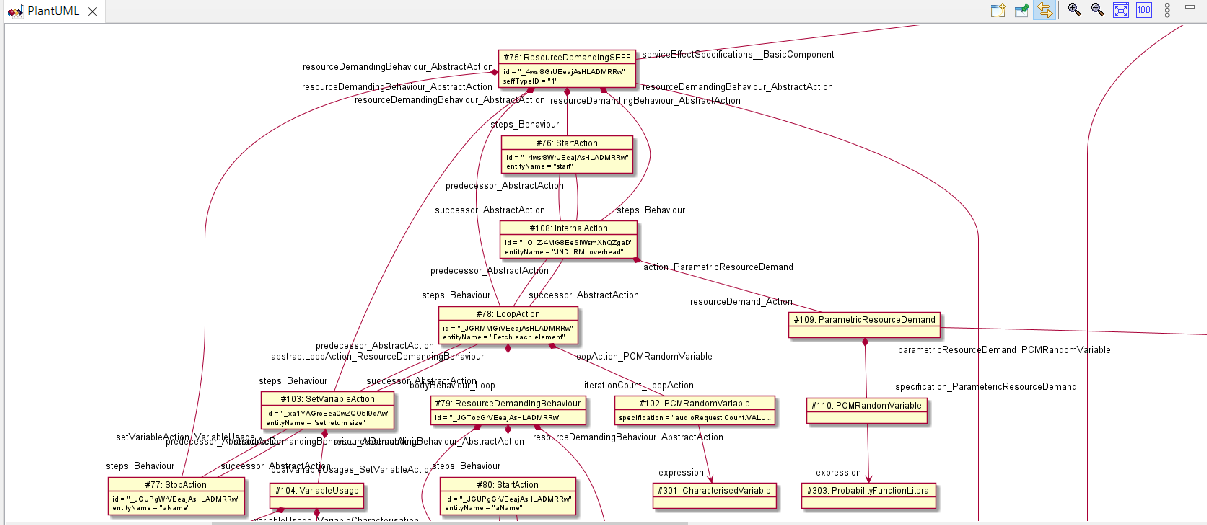
\includegraphics[width=\textwidth,height=1.1\textheight]{figures/motivation.png}
\end{frame}

\section{Grundlagen}
\subsection{Palladio}
\begin{frame}{Palladio Framework}
    \begin{columns}
        \column{.3\textwidth}
        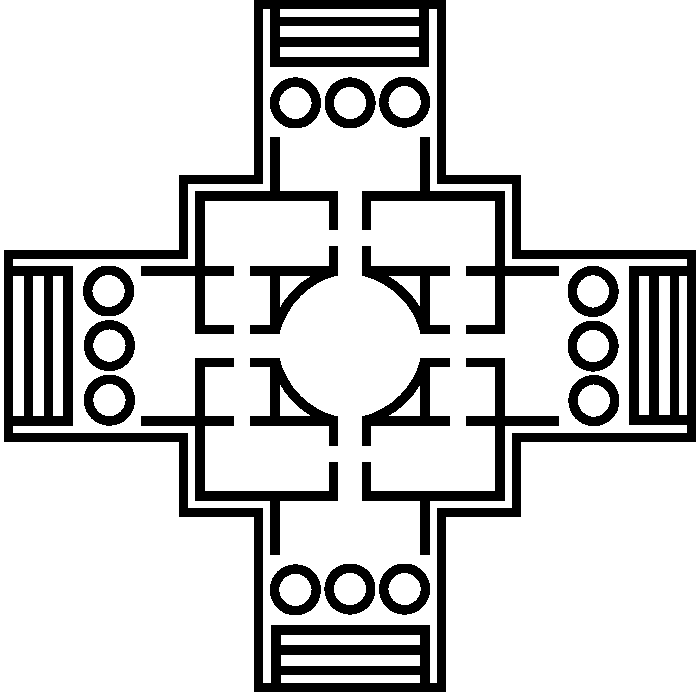
\includegraphics[width=\textwidth]{figures/palladio.pdf}
        \column{.7\textwidth}
        \begin{itemize}
            \item ...
            \item .
            \item ..
        \end{itemize}
    \end{columns}
\end{frame}
\begin{frame}
    \centering
    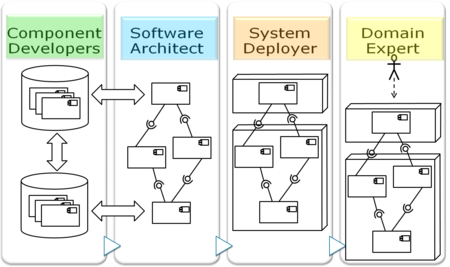
\includegraphics[width=.8\textwidth]{figures/palladio_sichten.png}
\end{frame}
\subsection{PlantUML}
\begin{frame}{PlantUML}
    \begin{columns}
        \column{.7\textwidth}
            \begin{itemize}
                \item Erstellen von UML Diagrammen durch textuelle Notation
                \item ein kurzes Beispiel?
                \item ...
            \end{itemize}
        \column{.3\textwidth}
            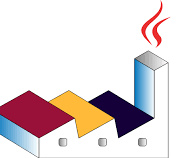
\includegraphics[width=\textwidth]{figures/plantuml.jpg}
    \end{columns}
\end{frame}


\section{Transformationen}
\subsection{Ansatz}
\begin{frame}{Ansatz}
    \begin{enumerate}
        \item Eigenes Bundle erstellen
        \item Eigene Klasse für jeden Diagrammtyp
        \item Durch die Palladio-Elemente iterieren -> in die textuelle PlantUML Notation "übersetzen"
        \item Hyperlinks (z.B zu Repository) hinzufügen
    \end{enumerate}
\end{frame}

\subsection{Architektur}
\begin{frame}{Architektur}
    auf einem Diagramm den Erweiterungspunkt zeigen
\end{frame}

\subsection{PlantUML Diagramme}
\begin{frame}{Repository-Diagramm}
    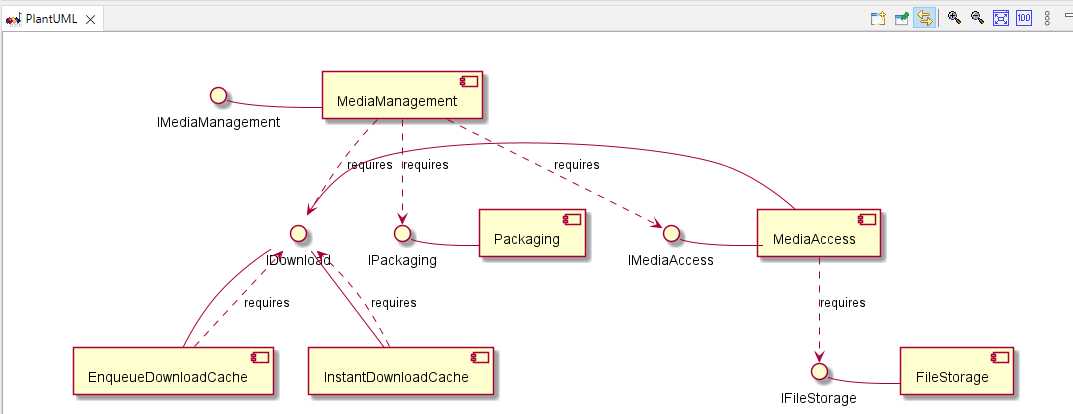
\includegraphics[width=\textwidth]{figures/repository.png}
\end{frame}
\begin{frame}{Systemdiagramm}
    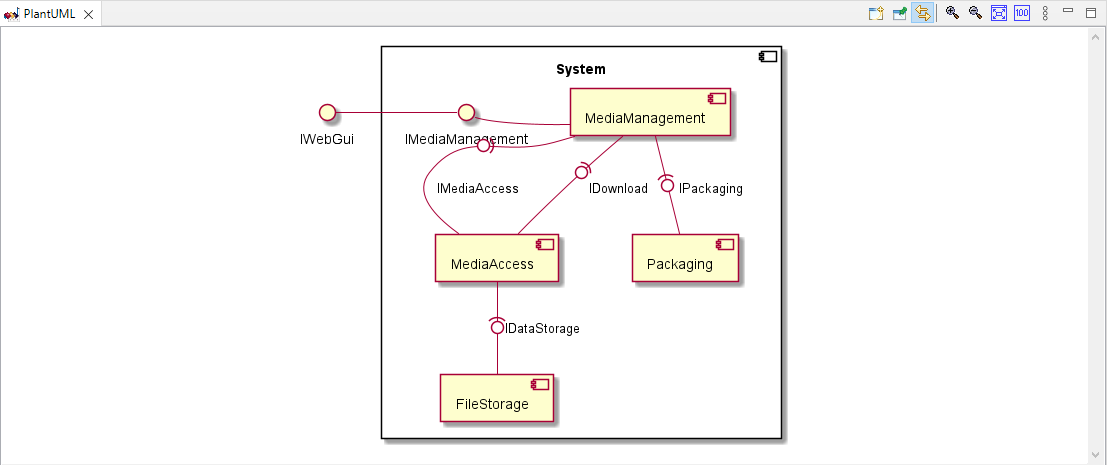
\includegraphics[width=\textwidth]{figures/system.png}
\end{frame}
\begin{frame}{Allocation-Diagramm}
    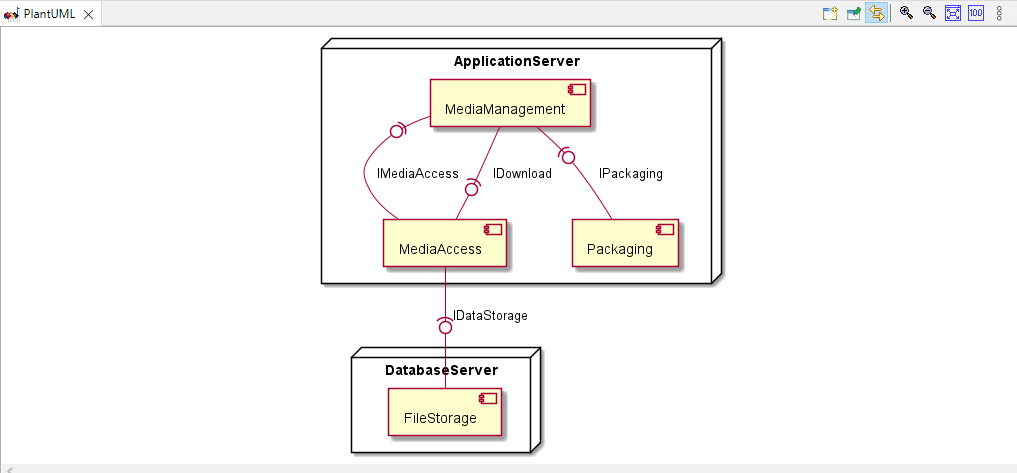
\includegraphics[width=\textwidth, height=.8\textheight]{figures/allocation.png}
\end{frame}

\section{Einschränkungen}
\begin{frame}{Einschränkungen}
 	\begin{redblock}{eins}
 		= \texttt{}
    \end{redblock}
     	\begin{redblock}{zwei}
 		= \texttt{}
    \end{redblock}
\end{frame}


\section{Zusammenfassung}
\begin{frame}{Zusammenfassung}
    
\end{frame}

\backupend

\end{document}
